%----------------------------------------------------------------------------------------
%	SOLUTION 3
%----------------------------------------------------------------------------------------
\subsection*{Solution 3}
\paragraph{Summary:} In the png image provided, there are total 4 channels, R, G, B and Alpha. The ranges for the values of these channels are $0-255$. As K-means is sensitive to the magnitudes of the vectors, I have normalized all the pixel values to $0-1$. At each iteration, cluster centers are initialized at random from uniform distribution over $0-1$. Also, I have use $10$ runs for each $k$ values and chosen the cluster means and labels of the run which produced lowest cumulative loss.

Reconstruction of the image is done as follows: If pixel $i$ belongs to cluster $C_k$, then in the reconstructed compressed image, value of pixel $i$ is replaced by the cluster mean $\mu_k$. Thus, reduction of many different pixel values to at most $k$ different values compresses the image.

\paragraph{Convergence Criteria:} I have used a tolerance of $1e-4$ in the decrease of cumulative loss between two consecutive iteration to declare convergence of the algorithm.

\paragraph{Results:} Fig.~\ref{fig:q3_loss_3}, \ref{fig:q3_loss_5} and \ref{fig:q3_loss_7} show the cumulative loss with iteration number in x-axis for $k=3,5$ and $7$ respectively. It can be seen that the cumulative loss when the algorithm converges is lowest for $k=7$ and highest for $k=3$. It can be interpreted that $k=7$ produces better reconstructed image at a cost of poor compression, while $k=3$ produces better compression at a cost of poor reconstruction.
%%%%%%%%%%%%%%%%%%%%%%% CUMULATIVE LOSS %%%%%%%%%%%%%%%%%%%%%
\begin{figure}[!h]
	\centering
	\subfloat[][K-means with $k=3$: Cumulative loss decreases with number of iterations]{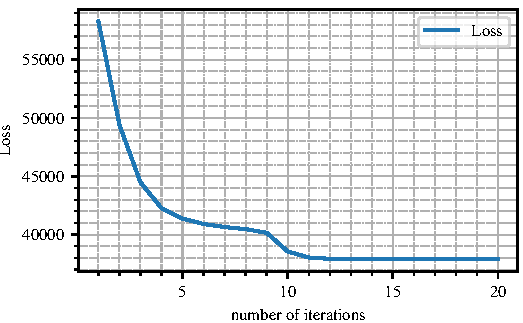
\includegraphics[scale=0.97,trim={0cm 0cm 0cm 0cm},clip]{./code/generatedPlots/q3_loss_3.pdf}\label{fig:q3_loss_3}}\hspace{0.5cm}
	\subfloat[][K-means with $k=5$: Cumulative loss decreases with number of iterations]{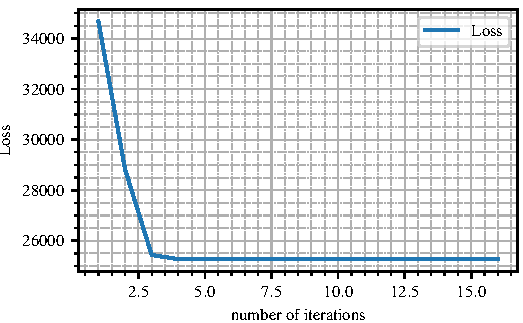
\includegraphics[scale=0.97,trim={0.0cm 0cm 0cm 0cm},clip]{./code/generatedPlots/q3_loss_5.pdf}\label{fig:q3_loss_5}}\hspace{0.5cm}
	\subfloat[][K-means with $k=7$: Cumulative loss decreases with number of iterations]{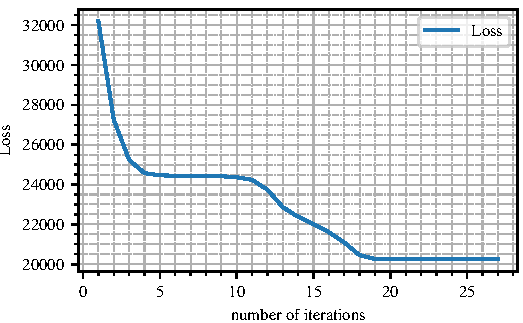
\includegraphics[scale=0.97,trim={0.0cm 0cm 0cm 0cm},clip]{./code/generatedPlots/q3_loss_7.pdf}\label{fig:q3_loss_7}}
	\caption{Q3: K-means: Cumulative loss with iteration number}
	\label{fig:q3_loss}
\end{figure}
Fig.~\ref{fig:compressed_img_3}, \ref{fig:compressed_img_5} and \ref{fig:compressed_img_7} show the reconstructed image after running K-means with $k=3,5$ and $7$ respectively. It can be seen that $k=7$ produces the best quality image and $k=3$ produces the lowest quality image.
%%%%%%%%%%%%%%%%%%%%%%% COMPRESSED IMAGE %%%%%%%%%%%%%%%%%%%%%
\begin{figure}[!h]
	\centering
	\subfloat[][Q3: K-means: Reconstructed image with $k=3$]{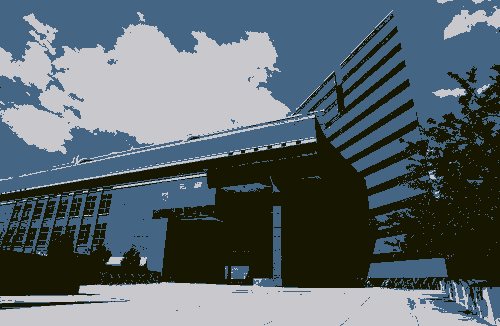
\includegraphics[scale=0.97,trim={0cm 0cm 0cm 0cm},clip]{./code/generatedPlots/compressed_img_3.png}\label{fig:compressed_img_3}}\hspace{0.5cm}
	\subfloat[][Q3: K-means: Reconstructed image with $k=5$]{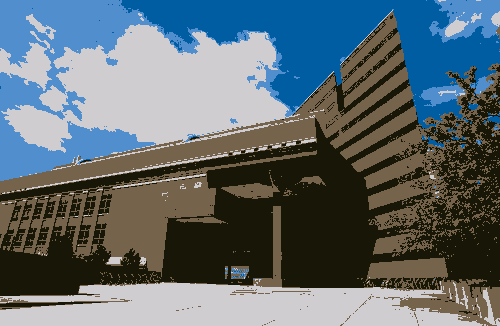
\includegraphics[scale=0.97,trim={0.0cm 0cm 0cm 0cm},clip]{./code/generatedPlots/compressed_img_5.png}\label{fig:compressed_img_5}}\hspace{0.5cm}
\end{figure}
\begin{figure}
	\ContinuedFloat
	\subfloat[][Q3: K-means: Reconstructed image with $k=7$]{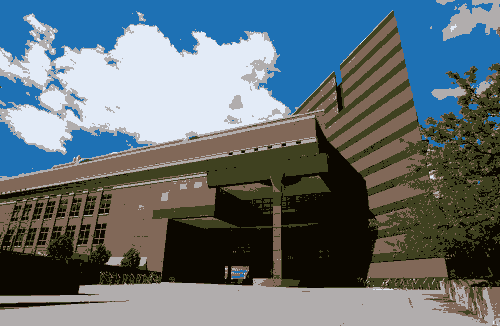
\includegraphics[scale=0.97,trim={0.0cm 0cm 0cm 0cm},clip]{./code/generatedPlots/compressed_img_7.png}\label{fig:compressed_img_7}}
	\caption{Q3: K-means: Reconstructed compressed image for different $k$ values}
	\label{fig:q3_compressed_img}
\end{figure}
